\chapter{Jet Results and Discussion} \label{ch:analysis}

Beginning in March of 2012, the LHC began seven months of pp collisions at $\sqrt{s} = \,$ 8 TeV.  The jet cross sections and ratios of the cross sections for jets of different radii offers a unique perspective on the pQCD effects of hadronization at this new energy frontier.  Due to the expectation that no QGP is formed in a pp collision these measurements serve as a baseline for separating phenomena associated with the QGP in heavy-ion collisions.  In order to measure the jet cross section the following formula is used,

\begin{equation}
	\frac{d \sigma^{jet}}{d\eta \, dp_{T}} = \frac{A_{trigger}}{\epsilon_{trigger}(p_{T})} \times C_{MC} \times \frac{1}{A(p_{T}) } \times \frac{1}{L_{int}} \times \frac{dN^{jet}}{dp_{T} \, d\eta}
\label{eq:xsecdef}
\end{equation}

\noindent
where,

\begin{itemize}
  \item $A_{trigger}$ is the acceptance for EMCal triggered events and $\epsilon_{trigger}(p_{T})$ is the EMCal trigger efficiency.  These factors correct for imperfections in the electronics of the EMCal and the overall factors are equal to one in minnimum bias events.
  \item $C_{MC}$ is a correction factor due to detector effects and it allows for comparisons between the ALICE experiment to other experiments or theoretical calculations.  Unfolding is used to determine this factor.
  \item $L_{int}$ is the integrated luminosity during the period when the data was recorded.
  \item $A(p_{T})$ is the geometrical detector acceptance.
  \item $\frac{dN^{jet}}{dp_{T} \, d\eta}$ is the inclusive jet momentum spectra.
  
\end{itemize}

\noindent
The following sections will go over how each factor was determined and the quality assurance procedures used for this analysis.

\section{Data Quality}
ALICE is a state-of-the-art experiment with excellent tracking and particle identification capabilities as discussed in Chapter \ref{ch:alice}.  However, just like any real world experiment, it contains a number of inefficiencies and imperfections.  This means that the data collected during the 8 TeV pp collision must be examined and any inaccuracies in the data must be removed before hard physics conclusions may be reached.  Data may be compromised at both the event-level, the experiment erroneously recorded something as an event, or at the constituent-level, one of the subdetectors mismeasured a feature of a particle, and these outliers must be accounted for and removed 
\section{Event Selection}

For an event to be selected into a physics analysis it must pass a number of quality control tests.  For example, the LHC must have be in a state of stable beams, cosmics must be excluded by only accepting tracks that originate from a vertex inside the detector, and the relevant detectors for a given analysis must be functioning as intended.  

\begin{figure}[h]
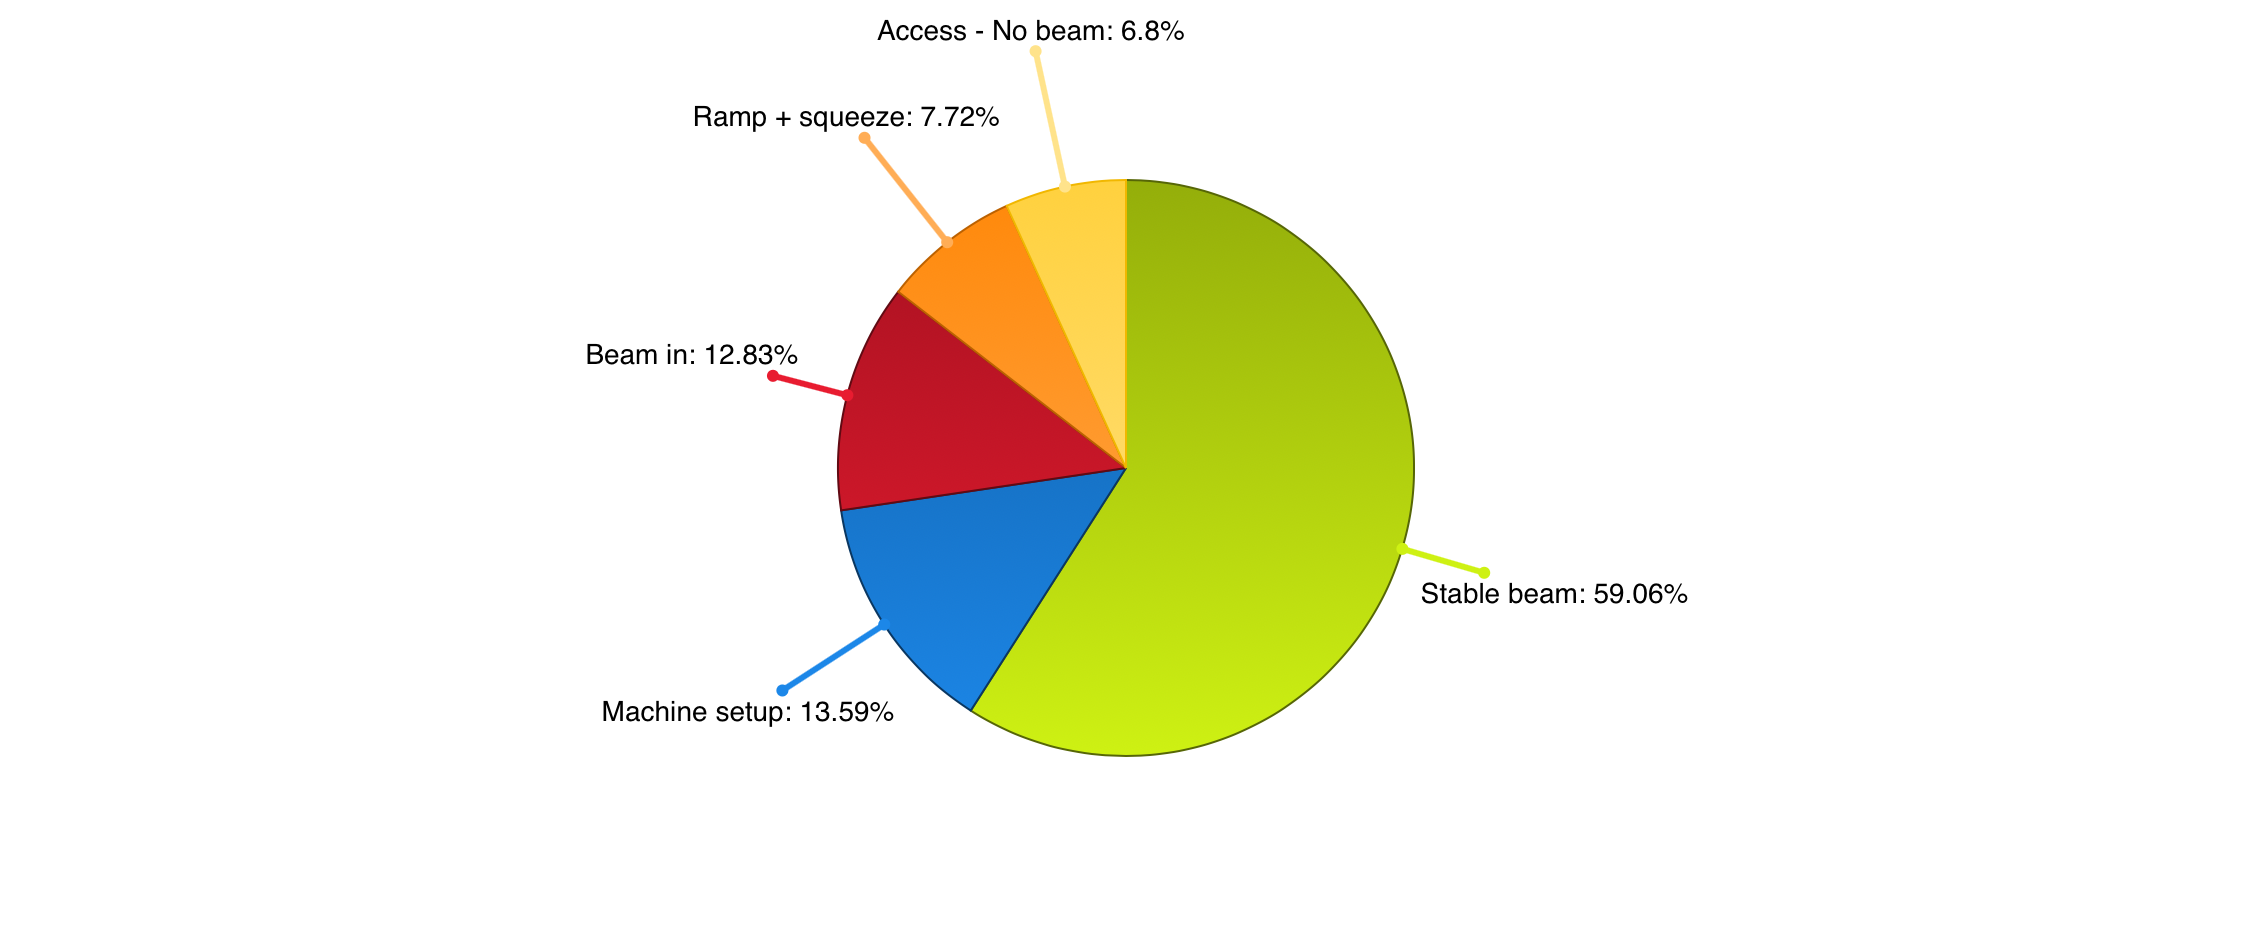
\includegraphics[width=17cm]{8TeVRunefficency}
\centering
\caption{LHC state during the 8 TeV run. }
\label{fig:RunEff}
\end{figure}

During the 8 TeV data collection period approximately 180 million minimum bias events were recorded, as summarized in table \ref{tab:RunSummary}.  These events are separated into periods, which dictate the particular beam and detector configurations during the data taking.The 8 TeV data is broken into 7 periods with approximately 181 million minimum bias events recorded.

\begin{table}[hb]
\label{tab:RunSummary}
\begin{center}
\begin{tabular}[b]{|c|c|c|}
	\hline
	Period & \# of runs & \# of Min Bias events \\ \hline
	LHC12c & 89 & $\sim \,$24 M \\ \hline
	LHC12d & 140 & $\sim \,$62 M \\ \hline
	LHC12e & 5 & $\sim \,$2 M \\ \hline
	LHC12f & 56 & $\sim \,$15 M \\ \hline
	LHC12g & 8 & $\sim \,$0.4 M \\ \hline
	LHC12h & 159 & $\sim \,$75 M \\ \hline
	LHC12i & 40 & $\sim \,$3 M \\ \hline
	Total & 497 & $\sim \,$181 M \\ \hline

\end{tabular}
\end{center}
\caption{2012 8 TeV data taking period.}
\end{table}

Approximatly, 15\% of the data sampled is unusable due to malfunctions in TPC chambers, EMCal super modules, the electronics for the EMCal or TPC, and   
\section{Raw measurements}
The ALICE experiment is capable of two types of jet reconstruction, charged and full jets.  Charged jets use information from the charged particle tracking detectors, such as the ITS and TPC, in conjunction with a jet finding algorithm to identify jets.  Full jets implement a similar procedure but also incorporates the EMCal in order to 

\subsection{Raw Jet Momentum Spectra in pp Collisions}

\section{Unfolding}

\subsection{Corrections to particle Level}

\subsection{Unfolding Matrix}

\subsection{Unfolded Spectra}

\section{Trigger Efficiency}

\section{Systematic Uncertainties}

\subsection{Systematic Uncertainty to Jet Yield}

\subsection{Systematic Uncertainty to Jet Energy Scale}

\subsection{Total Uncertainty}

\section{Corrected pp jet cross section}

\subsection{Comparisons to pQCD predictions}

\subsection{Jet Cross Section and Ratios}

Given two jets of different radii, $R_{1}$ and $R_{2}$, the ratio of the cross sections may be written in short hand as,

\begin{equation}
	\frac{\sigma_{R_{1}}}{\sigma_{R_{2}}}= \frac{d \sigma^{jet}_{R_{1}}}{d\eta \, dp_{T}} \Big/  \frac{d \sigma^{jet}_{R_{2}}}{d\eta \, dp_{T}}
\label{eq:xsecratiodef}
\end{equation}

